\subsection{Sample Data Insertion}

This section presents the consolidated sample data insertion script used by the group. 
The script combines the original sample data and the extended sample data so that all members can initialize and test the database with the same dataset.

The insertion script covers all tables in the Steam Store Management database, including users, players, developers, games, DLCs, promotions, transactions, ownership records, reviews, carts, achievements, and relationship tables. 
To avoid foreign key order issues during the insertion process, foreign key checks are temporarily disabled before inserting data and enabled again after all records have been inserted.

\subsubsection{Sample Data Coverage}

The inserted data represents realistic operations of a Steam-like digital distribution platform. 
The dataset includes player accounts, developer accounts, game products, downloadable content, promotions, purchase transactions, game ownership, DLC ownership, player reviews, carts, friends, and achievement records.

\begin{table}[H]
\centering
\caption{Summary of inserted sample data}
\label{tab:sample-data-summary}
\begin{tabular}{|l|r|p{7cm}|}
\hline
\textbf{Table} & \textbf{Rows} & \textbf{Description} \\ \hline
\texttt{USER} & 18 & User accounts including players and developers \\ \hline
\texttt{PLAYER} & 10 & Player profiles and wallet balances \\ \hline
\texttt{DEVELOPER} & 8 & Developer and publisher information \\ \hline
\texttt{CONTACT\_PHONE} & 8 & Developer contact phone numbers \\ \hline
\texttt{GENRE} & 5 & Game genre categories \\ \hline
\texttt{PROMOTION} & 7 & Discount campaigns and sale events \\ \hline
\texttt{GAME} & 11 & Game products published by developers \\ \hline
\texttt{DLC} & 10 & Downloadable content linked to games \\ \hline
\texttt{ACHIEVEMENT} & 5 & Game achievement records \\ \hline
\texttt{REVIEW} & 10 & Player reviews for games \\ \hline
\texttt{CART} & 5 & Player shopping carts \\ \hline
\texttt{TRANSACTION} & 15 & Completed purchase transactions \\ \hline
\texttt{FRIENDS} & 5 & Friendship relationships between players \\ \hline
\texttt{OWNS\_LIBRARY} & 5 & Player game ownership records \\ \hline
\texttt{CONTAINS} & 17 & Games included in purchase transactions \\ \hline
\texttt{GAME\_PROMOTION} & 5 & Game and promotion relationships \\ \hline
\texttt{GAME\_GENRE} & 13 & Game and genre relationships \\ \hline
\texttt{QUEUE} & 5 & Games temporarily stored in carts \\ \hline
\texttt{PLAYER\_ACHIEVEMENT} & 5 & Achievements unlocked by players \\ \hline
\texttt{BUY\_DLC} & 5 & DLC purchases in transactions \\ \hline
\texttt{OWNS\_DLC} & 5 & DLC ownership records \\ \hline
\end{tabular}
\end{table}
\subsubsection{Data Design Explanation}

The sample data is designed to support later testing of stored procedures, triggers, functions, and application interfaces. 
For example, the inserted users are divided into players and developers. 
Each game is linked to a developer, while DLC records are linked to their corresponding base games. 
Transactions are connected to players, and purchased games are recorded through the \texttt{CONTAINS} table. 
DLC purchases are represented through \texttt{BUY\_DLC}, while long-term ownership is represented through \texttt{OWNS\_LIBRARY} and \texttt{OWNS\_DLC}.

This dataset is meaningful because it does not only insert isolated records. 
Instead, the inserted records are connected through foreign key relationships and reflect realistic platform operations such as purchasing games, owning DLCs, reviewing games, adding games to carts, applying promotions, and unlocking achievements.
\subsubsection{Full SQL Data Insertion Script}

The following SQL script is the complete sample data insertion script used by the group.

\begin{lstlisting}[language=SQL, caption={Full SQL script for inserting sample data}, label={lst:insert-sample-data}]

SET FOREIGN_KEY_CHECKS = 0;

-- 1. USER TABLE
INSERT INTO `USER` (user_id, username, email, password_hash, join_date) VALUES
(1, 'khoitran', 'khoi.tran@gmail.com', 'hash1', '2023-01-15'),
(2, 'huylong', 'long.phan@gmail.com', 'hash2', '2023-02-20'),
(3, 'thanhnam', 'nam.pham@gmail.com', 'hash3', '2023-03-10'),
(4, 'thienan', 'an.trieu@gmail.com', 'hash4', '2023-04-05'),
(5, 'giahung', 'hung.nguyen@gmail.com', 'hash5', '2023-05-12'),
(6, 'riotgames', 'contact@riotgames.com', 'dev1', '2020-10-01'),
(7, 'cd_projekt', 'hello@cdprojekt.com', 'dev2', '2019-11-11'),
(8, 'valve_corp', 'support@valvesoftware.com', 'dev3', '2018-05-20'),
(9, 'mihoyo', 'business@mihoyo.com', 'dev4', '2021-06-15'),
(10, 'vng_games', 'admin@vng.com.vn', 'dev5', '2015-08-08'),
(11, 'faker_vn', 'faker.vn@gmail.com', 'hash11', '2023-06-01'),
(12, 'mixigaming', 'do.mixi@gmail.com', 'hash12', '2023-07-15'),
(13, 'crisdevil', 'cris.phan@gmail.com', 'hash13', '2023-08-20'),
(14, 'phuongly', 'ly.phuong@gmail.com', 'hash14', '2023-09-10'),
(15, 'sontungmtp', 'mtp.ent@gmail.com', 'hash15', '2023-10-05'),
(16, 'rockstar_games', 'contact@rockstargames.com', 'dev16', '2015-01-01'),
(17, 'square_enix', 'info@square-enix.com', 'dev17', '2016-02-02'),
(18, 'capcom_ltd', 'support@capcom.co.jp', 'dev18', '2017-03-03');

-- 2. PLAYER TABLE
INSERT INTO `PLAYER` (user_id, wallet_balance, profile_bio) VALUES
(1, 500000.0, 'Yasuo main, 20 games per day'),
(2, 1000000.0, 'Passionate about RPG games'),
(3, 50000.0, 'Plays games to relieve stress'),
(4, 250000.0, 'FPS sharpshooter'),
(5, 0.0, 'Free-to-play grinder, never tops up'),
(11, 1500000.0, 'Pro boosting player'),
(12, 5000000.0, 'Auto Chess legend'),
(13, 2000000.0, 'Casual game reviewer'),
(14, 500000.0, 'Plays mostly for fun'),
(15, 10000000.0, 'Whale, top-up king');

-- 3. DEVELOPER TABLE
INSERT INTO `DEVELOPER` (user_id, legal_name, bank_account) VALUES
(6, 'Riot Games Inc.', 'BANK_123'),
(7, 'CD Projekt S.A.', 'BANK_987'),
(8, 'Valve Corporation', 'BANK_111'),
(9, 'miHoYo Co., Ltd.', 'BANK_444'),
(10, 'VNG Corporation', 'BANK_777'),
(16, 'Rockstar Games', 'BANK_RSTAR'),
(17, 'Square Enix Co., Ltd.', 'BANK_SQEX'),
(18, 'Capcom Co., Ltd.', 'BANK_CAPCOM');

-- 4. CONTACT_PHONE TABLE
INSERT INTO `CONTACT_PHONE` (developer_user_id, contact_phone) VALUES
(6, '+1-800-555-0101'),
(7, '+48-22-123-4567'),
(8, '+1-800-555-0202'),
(9, '+86-21-1234-5678'),
(10, '+84-28-3962-3688'),
(16, '+1-800-RSTAR-01'),
(17, '+81-3-5292-8100'),
(18, '+81-6-6920-3600');

-- 5. GENRE TABLE
INSERT INTO `GENRE` (genre_name, description) VALUES
('Action', 'Action games'),
('RPG', 'Role-playing games'),
('FPS', 'First-person shooter'),
('MOBA', 'Multiplayer online battle arena'),
('Strategy', 'Strategy games');

-- 6. PROMOTION TABLE
INSERT INTO `PROMOTION` (promotion_id, name, discount_percentage, start_date, end_date) VALUES
(1, 'Summer Sale', 50.0, '2026-06-01', '2026-06-30'),
(2, 'Winter Sale', 70.0, '2026-12-15', '2026-12-31'),
(3, 'Black Friday', 80.0, '2026-11-25', '2026-11-30'),
(4, 'Lunar New Year', 30.0, '2026-02-10', '2026-02-20'),
(5, 'Weekend Deal', 15.0, '2026-04-18', '2026-04-20'),
(6, 'Halloween Sale', 60.0, '2026-10-25', '2026-11-01'),
(7, 'Spring Festival', 40.0, '2026-03-15', '2026-03-25');

-- 7. GAME TABLE
INSERT INTO `GAME` (game_id, title, base_price, release_date, graphics, os, processor, memory, developer_id) VALUES
(1, 'League of Legends', 0.0, '2009-10-27', 'GTX 1050', 'Windows 10', 'Intel i3', '8GB RAM', 6),
(2, 'Valorant', 0.0, '2020-06-02', 'GTX 1050 Ti', 'Windows 10', 'Intel i5', '8GB RAM', 6),
(3, 'Cyberpunk 2077', 990000.0, '2020-12-10', 'RTX 3060', 'Windows 11', 'Intel i7', '16GB RAM', 7),
(4, 'Half-Life: Alyx', 1200000.0, '2020-03-23', 'GTX 1060', 'Windows 10', 'Intel i5', '12GB RAM', 8),
(5, 'Genshin Impact', 0.0, '2020-09-28', 'GTX 1060', 'Windows 10', 'Intel i5', '8GB RAM', 9),
(6, 'Grand Theft Auto V', 500000.0, '2015-04-14', 'GTX 660', 'Windows 10', 'Intel i5', '8GB RAM', 16),
(7, 'Red Dead Redemption 2', 1000000.0, '2019-11-05', 'GTX 1060', 'Windows 10', 'Intel i7', '12GB RAM', 16),
(8, 'Final Fantasy VII Remake', 1500000.0, '2021-12-16', 'RTX 2060', 'Windows 10', 'Intel i7', '16GB RAM', 17),
(9, 'Resident Evil 4', 1200000.0, '2023-03-24', 'RX 5600 XT', 'Windows 11', 'Ryzen 5', '16GB RAM', 18),
(10, 'Monster Hunter: World', 600000.0, '2018-08-09', 'GTX 1060', 'Windows 10', 'Intel i5', '8GB RAM', 18),
(11, 'The Witcher 3: Wild Hunt', 400000.0, '2015-05-18', 'GTX 770', 'Windows 10', 'Intel i5', '8GB RAM', 7);

-- 8. DLC TABLE
INSERT INTO `DLC` (game_id, dlc_name, price, release_date) VALUES
(3, 'Phantom Liberty', 450000.0, '2023-09-26'),
(1, 'Arcane Jinx Skin', 200000.0, '2024-11-01'),
(5, 'Moonlight Blessing', 109000.0, '2020-10-01'),
(2, 'Prime Vandal Bundle', 300000.0, '2021-05-15'),
(4, 'Soundtrack Collection', 150000.0, '2020-04-10'),
(6, 'Criminal Enterprise Starter Pack', 200000.0, '2017-12-15'),
(8, 'EPISODE INTERmission', 400000.0, '2021-12-16'),
(9, 'Separate Ways', 250000.0, '2023-09-21'),
(10, 'Iceborne Expansion', 500000.0, '2020-01-09'),
(11, 'Blood and Wine', 200000.0, '2016-05-31');

-- 9. ACHIEVEMENT TABLE
INSERT INTO `ACHIEVEMENT` (game_id, achievement_name, points, description) VALUES
(1, 'Penta Kill', 100, 'Eliminate 5 enemy champions in a row'),
(3, 'The Star', 50, 'Complete The Star ending'),
(4, 'Gnome Chompski', 200, 'Bring the Gnome statue to the bunker'),
(5, 'Abyss Floor 12', 150, 'Clear floor 12 of the Spiral Abyss'),
(2, 'Ace', 100, 'Single-handedly eliminate all enemies');

-- 10. REVIEW TABLE
INSERT INTO `REVIEW` (rating, comment, review_date, player_id, game_id) VALUES
('Recommended', 'Extremely addictive game!', '2024-01-10', 1, 3),
('Recommended', 'Good game but a bit laggy', '2024-02-12', 2, 1),
('Recommended', 'Top-tier VR experience', '2024-03-15', 3, 4),
('Not Recommended', 'Gacha rates are too brutal', '2024-04-20', 4, 5),
('Recommended', 'Best tactical shooter, hands down', '2024-05-25', 5, 2),
('Recommended', 'Masterpiece open world!', '2024-05-20', 11, 7),
('Recommended', 'Stunning graphics, great storyline', '2024-05-25', 12, 8),
('Recommended', 'Gwent is more fun than the main quest', '2024-06-05', 13, 11),
('Not Recommended', 'Ashley screaming for help is deafening', '2024-06-15', 14, 9),
('Recommended', 'Fun grindy game', '2024-07-10', 15, 10);

-- 11. CART TABLE
INSERT INTO `CART` (cart_id, last_updated, player_id) VALUES
(1, '2026-04-15 10:00:00', 1),
(2, '2026-04-16 11:30:00', 2),
(3, '2026-04-17 14:45:00', 3),
(4, '2026-04-18 09:15:00', 4),
(5, '2026-04-19 20:20:00', 5);

-- 12. TRANSACTION TABLE
INSERT INTO `TRANSACTION` (transaction_id, date, payment_method, total_amount, player_id) VALUES
(1, '2023-12-25 08:30:00', 'Credit Card', 990000.0, 1),
(2, '2024-01-05 14:20:00', 'Momo', 1200000.0, 2),
(3, '2024-02-14 19:45:00', 'ZaloPay', 450000.0, 1),
(4, '2024-03-08 21:10:00', 'PayPal', 109000.0, 4),
(5, '2024-04-01 10:05:00', 'Credit Card', 200000.0, 2),
(6, '2024-05-10 10:00:00', 'Momo', 1500000.0, 11),
(7, '2024-05-15 14:30:00', 'Credit Card', 2200000.0, 12),
(8, '2024-06-01 09:15:00', 'ZaloPay', 600000.0, 13),
(9, '2024-06-10 20:45:00', 'PayPal', 1700000.0, 14),
(10, '2024-07-05 11:20:00', 'Credit Card', 200000.0, 15),
(11, '2024-07-20 16:00:00', 'Momo', 1200000.0, 1),
(12, '2024-08-15 08:30:00', 'Momo', 400000.0, 2),
(13, '2024-09-01 19:10:00', 'ZaloPay', 1500000.0, 3),
(14, '2024-10-31 22:00:00', 'Credit Card', 500000.0, 4),
(15, '2024-11-26 23:59:00', 'PayPal', 1000000.0, 5);

-- 13. FRIENDS TABLE
INSERT INTO `FRIENDS` (player_id, friend_id) VALUES
(1, 2), (1, 3), (2, 4), (3, 5), (4, 5);

-- 14. OWNS_LIBRARY TABLE
INSERT INTO `OWNS_LIBRARY` (player_id, game_id, purchase_date, total_playtime) VALUES
(1, 3, '2023-12-25', 120),
(1, 2, '2023-12-25', 500),
(2, 4, '2024-01-05', 45),
(4, 5, '2024-03-08', 300),
(2, 1, '2024-04-01', 1000);

-- 15. CONTAINS TABLE
INSERT INTO `CONTAINS` (transaction_id, game_id, price_at_purchase) VALUES
(1, 3, 990000.0),
(2, 4, 1200000.0),
(4, 5, 0.0),
(5, 1, 0.0),
(1, 2, 0.0),
(6, 7, 1000000.0),
(6, 6, 500000.0),
(7, 8, 1500000.0),
(7, 10, 600000.0),
(8, 11, 400000.0),
(9, 9, 1200000.0),
(10, 8, 1500000.0),
(11, 9, 1200000.0),
(12, 11, 400000.0),
(13, 7, 1000000.0),
(14, 6, 500000.0),
(15, 7, 1000000.0);

-- 16. GAME_PROMOTION TABLE
INSERT INTO `GAME_PROMOTION` (game_id, promotion_id) VALUES
(3, 1), (4, 2), (3, 3), (5, 4), (1, 5);

-- 17. GAME_GENRE TABLE
INSERT INTO `GAME_GENRE` (game_id, genre_name) VALUES
(1, 'MOBA'), (2, 'FPS'), (3, 'RPG'), (3, 'Action'), (4, 'FPS'),
(6, 'Action'), (7, 'Action'), (7, 'RPG'), (8, 'RPG'), (9, 'Action'),
(10, 'RPG'), (10, 'Action'), (11, 'RPG');

-- 18. QUEUE TABLE
INSERT INTO `QUEUE` (cart_id, game_id) VALUES
(1, 3), (1, 4), (2, 5), (3, 1), (5, 2);

-- 19. PLAYER_ACHIEVEMENT TABLE
INSERT INTO `PLAYER_ACHIEVEMENT` (player_id, game_id, achievement_name, unlock_date) VALUES
(1, 3, 'The Star', '2024-01-20'),
(2, 4, 'Gnome Chompski', '2024-02-10'),
(4, 5, 'Abyss Floor 12', '2024-03-25'),
(1, 2, 'Ace', '2023-12-30'),
(2, 1, 'Penta Kill', '2024-05-01');

-- 20. BUY_DLC TABLE
INSERT INTO `BUY_DLC` (transaction_id, game_id, dlc_name, purchase_date) VALUES
(3, 3, 'Phantom Liberty', '2024-02-14'),
(5, 1, 'Arcane Jinx Skin', '2024-04-01'),
(4, 5, 'Moonlight Blessing', '2024-03-08'),
(1, 2, 'Prime Vandal Bundle', '2023-12-25'),
(2, 4, 'Soundtrack Collection', '2024-01-05');

-- 21. OWNS_DLC TABLE
INSERT INTO `OWNS_DLC` (player_id, game_id, dlc_name, purchase_date) VALUES
(1, 3, 'Phantom Liberty', '2024-02-14'),
(2, 1, 'Arcane Jinx Skin', '2024-04-01'),
(4, 5, 'Moonlight Blessing', '2024-03-08'),
(1, 2, 'Prime Vandal Bundle', '2023-12-25'),
(2, 4, 'Soundtrack Collection', '2024-01-05');

SET FOREIGN_KEY_CHECKS = 1;
\end{lstlisting}
\subsubsection{Execution Result}

After executing the sample data insertion script, the number of inserted records was verified using \texttt{COUNT(*)} queries for all tables. 
The result in Figure~\ref{fig:sample-data-count-result} shows that all main entity tables and relationship tables contain data and are ready for testing later database operations.

\begin{figure}[H]
    \centering
    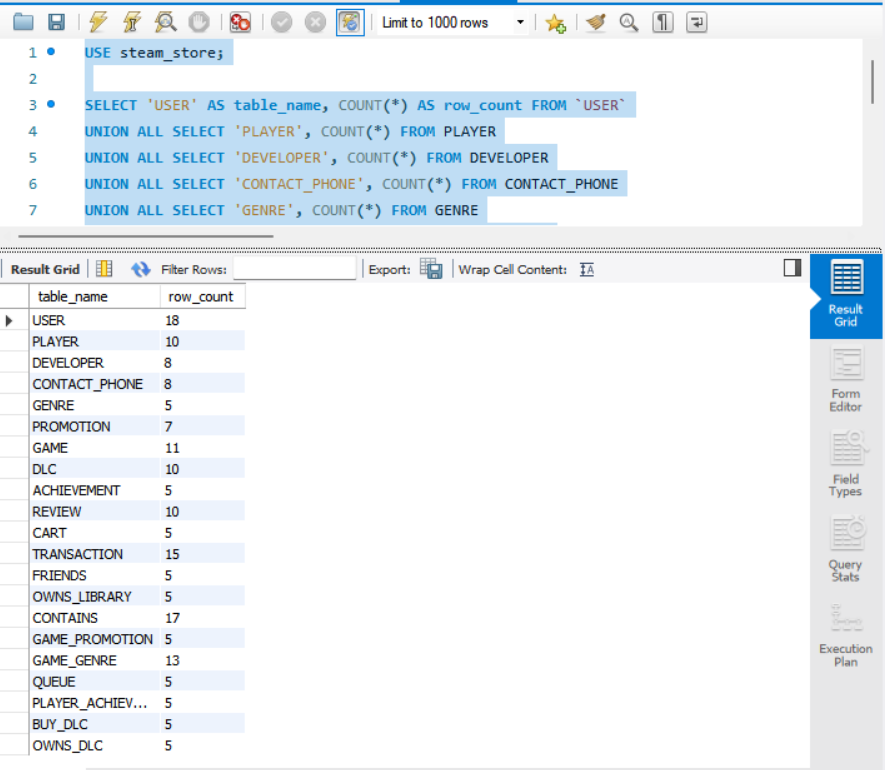
\includegraphics[width=0.9\linewidth]{graphics/sample-data-count-result.png}
    \caption{Verification of inserted sample data using row count queries}
    \label{fig:sample-data-count-result}
\end{figure}
